%Se abre la veda. Sin piedad con él paper!

\documentclass{llncs}
\usepackage{graphics}
\usepackage[dvips]{epsfig}
\usepackage[latin1]{inputenc}
\usepackage{color}
\usepackage{longtable}
%\usepackage{multirow}
\usepackage[dvips]{graphicx} 
%\usepackage{amsmath}
\usepackage{textcomp}
\usepackage{url}
\usepackage{algpseudocode}
\usepackage{caption}
\usepackage{subcaption}

\captionsetup{compatibility=false}

\newcommand{\tab}{\hspace{20mm}}

\setlength{\textfloatsep}{8pt plus 2pt minus 2pt}
\setlength{\intextsep}{8pt plus 2pt minus 2pt}

%#\def\BibTeX{{\rm B\kern-.05em{\sc i\kern-.025em b}\kern-.08em
%#    T\kern-.1667em\lower.7ex\hbox{E}\kern-.125emX}}

%\hyphenation{}

\begin{document}

%%%%%%%%%%%%%%%%%%%%%%%%%%%%%%%   TITLE   %%%%%%%%%%%%%%%%%%%%%%%%%%%%%%%

\title{Co-Evolutionary Optimization of Autonomous Agents in a Real-Time Strategy Game}
% autonomous por qué? Por qué no simplemente playing?

%OK, no revisamo0s, pero para eso mejor haz una rama y trabaja con la
%rama. No cambies nombres que despista. - JJ

\titlerunning{Co-Evolutionary Optimization of Bots in an RTS}


%%%%%%%%%%%%%%%%%%%%%%%%%%%%%%%   AUTHORS   %%%%%%%%%%%%%%%%%%%%%%%%%%%%%%%

%\author{A. Fernández-Ares \and A.M. Mora \and  J.J. Merelo \and \\ P. García-Sánchez \and P.A. Castillo}
%\authorrunning{A. Fernández-Ares. et al.}
%
%\institute{Departamento de Arquitectura y Tecnolog\'{\i}a de Computadores.\\
%Universidad de Granada (Spain)\\
%\email{antares.es@gmail.com}, \\ \email{\{amorag,jmerelo,pgarcia,pedro\}@geneura.ugr.es}
%}

\maketitle

%
%%%%%%%%%%%%%%%%%%%%%%%%%%%%%%%   ABSTRACT   %%%%%%%%%%%%%%%%%%%%%%%%%%%%%%%
%
\begin{abstract}
This paper presents an approach based in an evolutionary algorithm
(EA), aimed to improve the behavioral parameters which guide the
actions of an autonomous agent (bot) inside a real-time strategy game
(RTS) named Planet Wars. 

Specifically the work describes a co-evolutionary implementation of a
previously presented method, which yielded successful results.
Thus, it's analyzed the effects of considering several individuals
to be evolved (improved) at the same time in the algorithm,
the use of 3 different fitness for measure the goodness of each bot in the evaluation,
and the variance of use an EA with and without previous knowledge for the training.

To this end, 4 on 4 matches have been considered. Two variants are presented:
without previous knowledge (where the 4 bots belong to the population) and with
(2 bots of the population versus 2 previously studied with good results bots).

For the fitness, 3 methods are studied: one based in turns and result position,
and another two based in the survey of the percentage of ships that belong each bot in each turn of the battle, using linear regression and area calculus. 

In this paper we set several goals for the uses of the co-evolution:
reduce the time needed for training in behavior with a huge time of evaluation,
improve best bots for used in 4 on 4 battles,
studies the significant different between the training with and without previous knowledge
and finally studies alternatives fitness for co-evaluations.

\end{abstract}

%
%%%%%%%%%%%%%%%%%%%%%%%%%%%%%%%   INTRODUCTION   %%%%%%%%%%%%%%%%%%%%%%%%%%%%%%%
%
\section{Introduction}
\label{sec:intro}
%







%En un track de juegos, no puedes empezar justificando la
%investigación en juegos. Habla de por qué usas coevolución o, si
%acaso, el interés que puede tener mejorar bots (puede haber gente de
%juegos de mesa o de cartas) - JJ
Autonomous agents (or \textit{bots}) in videogames have become very popular in the last years, because they can increase the challenge and lasting appeal of the game, by competing or cooperating with the human player.
% Maribel: tal y como dice J, podrías decir justo lo mismo, pero de enfoques coevolutivos, puedes referenciar algoritmos coevolutivos recientes en varios ámbitos
Thus, designing a good behavioural engine for them is one of the main
topics of interest in the actual videogame development task.
% ¿Qué significa good en este caso? ¿Asesino? - JJ
They have been widely used in Fisrt Person Shooter games (FPSs) % Falta una referencia a FPSs
from the nineties, but in this paper we will % Maribel- no uses futuro, en español se usa el futuro, pero en inglés el paper se cuenta en presente o en pasado y en cualquier caso, nunca mezclandolo con futuro. Cuando escribes el paper, ya lo has hecho, no es futuro.
work with them on a Real-Time Strategy game (RTS).
RTSs are a sub-genre of strategy-based video games in which the contenders control a set of units and structures distributed in a playing area and combat using them for conquering the scenario or defeating the opponent.
Command and Conquer\texttrademark,
Starcraft\texttrademark, Warcraft\texttrademark~ and Age of
Empires\texttrademark~ are some examples of these type of games.   

%RTS games often employ two levels of AI: the
%first one, makes decisions on the set of units (workers, soldiers, machines,
%vehicles or even buildings); the second level is devoted to every one of
%these small units. These two level of actions, which can be considered
%{\em strategical} and {\em tactical}, make them inherently difficult;
%but they are made even more so due to their real-time nature (usually addressed by constraining the time that can be used to make a decision) and also for the huge search space (plenty of possible behaviours) that is implicit in its action.
The RTS considered % Maribel, ves, aquí vuelves a usar pasado 
in the paper 
% Maribel- Sólo en el paper, en otro sitio no se llama así?
in named \textit{Planet Wars}, and it was used a platform in the Google AI Challenge 2010. % Maribel, a esta frase anterior le falta algo, un in quizás?
In this contest, `real time' is sliced in one second \textit{turns}, with players receiving the chance to play sequentially. However, \textit{actions} happen at the \textit{simulated} same time. 

% Hala, salto. Pasas de describir qué juego a decir qué haces. Métela
% poquito a poco: hicimos esto, funcionó regular porque no teníamos
% más que no sé cuantos oponentes, vamos a hacerlo de esta forma
% porque no sé quién dijo que era muy guay - JJ 
% Maribel- Ahora hablas en presente, menudo ?ío!!
This paper describes a Co-Evolutionary \cite{Coevolution95} approach
for improving % mejorar con respecto a qué? - JJ
the decision engine of a bot that plays that RTS. This engine consists
in a set of rules previously designed and evolved by the authors in
\cite{Genebot_CEC11} % recordad doble ciego, anonimizar - JJ
, using an % Maribel- el an sobra, debería ser a
regular Genetic Algorithm (GA) \cite{GAs_Goldberg89}. We
applied an offline evolution (i.e., not during the match, but prior to
the game battles) of the parameters on which the behavioural rules
depends. 

The evaluation of the quality (fitness) of each set of rules in the
population was made by playing the bot against predefined opponents, being a pseudo-stochastic or \textit{noisy} function, since the results for the same individual evaluation may change from time to time, yielding good or bad values depending on the battle events and on the opponent's actions. We have dealt with this noisy nature \cite{genebot-evo12} % Maribel- revisión doble ciega otra vez aquí 
by means of a reevaluation phase of all the individuals every generation, along with an average calculation of the fitness value of every individual after five combats (in five different an representative maps). %Maribel- Pon el criterio con el que has elegido los mapas, por qué esos y no otros.

The aim is that the co-evolutionary scheme improves the fitness
convergence of the population, since the individuals cooperate in
their evolution. % lo uno no se sigue de lo otro, explicar el
                 % argumento - JJ
                 
% Maribel- Deberías decir algo de por qué el enfoque anterior no era bueno y por qué has decidido hacerlo coevolutivo, es decir que si
% el otro se estancaba, por qué se estancaba y en qué casos y así concluir poco a poco que un enfoque coevolutivo mejoraría esos %problemas previos 
 Thus, we have  considered  matches with four players, with two of the
 contenders the individuals being evolved at a specific generation,
 and the other two opponents with a fixed AI engine, namely the
 competition sparring \textit{GoogleBot} in one of the experiments,
 and our best individual to date, baptised as \textit{Genebot-8}, in
 the other one.  
 % Maribel- Esto creo que debería estar en el apartado de experimentos
 
%Estás explicando la metodología antes de tiempo. Tienes que
%justificar por qué usas coevolución y qué pistas tienes de que los
%resultados serían mejores - JJ

%In the experiments, we will show that the set of rules evolve towards better bots, and finally an efficient player is returned by the GA. 
%In addition, several experiments have been conducted to analyse the issue of the cited \textit{noisy fitness} in this problem.
%The experiments show its presence, but also the good behaviour of the chosen fitness function to deal with it and yield good individuals even in these conditions. 

% ¿esto por qué lo borras - JJ 
%The paper is structured as follows: 
%The next section reviews related approaches to behavioural engine design in similar game-based problems. 
%Section \ref{sec:planet_wars} addresses the problem by describing the game of Planet Wars.  
%Section \ref{sec:genebot} presents the proposed method, termed {GeneBot}, starting from the initial approach, and the GA used to evolve the behaviour. 
%The experiments and results are described and discussed in Section \ref{sec:experiments}. Finally, the conclusions and future lines of research are presented in Section \ref{sec:conclusions}.

%%%%%%%%%%%%%%%%%%%%%%%%%%%%%%  STATE OF THE ART  %%%%%%%%%%%%%%%%%%%%%%%%%%%%%
%
\section{State of the Art}
\label{sec:stateofart}
%

Video games have become one of the biggest sectors in the
entertainment industry; after the previous phase of searching for the
graphical quality perfection, the players now request opponents
exhibiting intelligent behaviour, or just human-like behaviours
\cite{artifical-stupidity-game-wisdom2-2004}. % irrelevante en el
                                % contexto. Tienes que empezar
                                % enmarcando el juego y las técnicas
                                % usadas: algoritmos genéticos, RTS,
                                % coevolución aplicado a unos y otros
                                % - JJ

%Nowadays, the games AI research has followed a different path, mainly starting with the improvement of FPS Bot's AI with Doom\texttrademark~ or
%Quake\texttrademark~ by the beginning of the 90s; and the most famous environment inside this kind of games, Unreal Tournament \texttrademark~\cite{Agent_Smith_CEC2009,ControllingBot_CEC2010,cooperativebots_CIG2010}.

Most of the researches have been done on relatively simple games such
as Super Mario \cite{Togelius_SuperMario}, Pac-Man
\cite{Pac-MAnt_CIG2010} or Car Racing Games \cite{CarRacing_Pelta09},
being many bots competitions involving them. % Vale, todo el mundo es
                                % un pringao y usa juegos simples, de
                                % estas te meten una hostia tus
                                % compañeros de sesión. Basta con que
                                % digas simplemente que los RTS tienen
                                % un enfoque diferente a estos juegos
                                % - JJ

RTS games show an emergent component \cite{emergence_in_games2008} as a consequence of the cited two level AI, since the units behave in many  % maribel- Many different es redundante, pon sólo many 
(and sometimes unpredictable) ways. This feature can make a RTS game more entertaining for a player and maybe more interesting for a researcher.
There are many research problems with regard to the AI for RTSs, % no uses with regard, pon regarding
including planning in an uncertain world with incomplete information;
learning; opponent modelling and spatial and temporal reasoning
\cite{hongchoCIG2005}. 

However, the reality in the industry is that in most of the RTS games,
the bot is  controlled by a fixed script that has been previously
programmed (following a finite state machines or a decision tree, for
instance). % tampoco me sirve a estas alturas. Hay miles de trabajos
           % de RTS- CI Justifica las técnicas usadas, no que vayas a
           % usar ese tipo de juego - JJ
Once the user has learnt how such a game will react, the game
becomes less interesting to play. In order to improve the users' gaming
experience, some authors such as Falke et al. \cite{falke2003} proposed a learning classifier system that can be used to endow the computer with
dynamically-changing %Maribel- por qué le pones el guión, quitaselo, dice lo mismo y esa palabra no existe como tal
strategies that respond to the user's strategies,
thus greatly extending the games playability. % Vale, seguimos
                                % justificando el uso de CI en juegos
                                % en un congreso de CI en juegos. - JJ
%Moreover, some authors have research the implementation of a human-like AI \cite{weber2011-humanlevelAI}.

In addition, in many RTS games, traditional artificial intelligence techniques fail to play at a human level because of the vast search spaces that they entail \cite{Aha05learningtowin}. In this sense, Ontano et at. \cite{ontanon2007} proposed to extract behavioural knowledge from expert demonstrations in form of individual cases. This knowledge could be reused via a case-based behaviour
generator that proposed advanced behaviours to achieve specific
goals. %Irrelevante para el trabajo - JJ 

%In this line there are several works dealing with the case-base reasoning such as Baumgarten et al. \cite{Baumgarten-combiningAImethods} that combines some AI techniques, or Palma et al. \cite{Palma-behaviortrees} who apply behaviour trees.

%Recently a number of soft-computing techniques and algorithms, such as co-evolutionary algorithms \cite{co-evol-rts2006} or multi-agent based methods \cite{HagelbackJ09}, just to cite a few, have already been applied to handle these problems in the implementation of RTS games. For instance, there are many benefits attempting to build adaptive learning AI systems which may exist at multiple levels of the game hierarchy, and which co-evolve over time. 
%In these cases, co-evolving strategies might be not only opponents but also partners coperating at different levels \cite{Livingstone05}.
%Other authors propose using co-evolution for evolving team tactics
%\cite{avery2010coevolving}. However, the problem is how tactics are
%constrained and parametrised and how the overall score is computed. 

% Las carencias de estrategias tradicionales han llevado a... Un
% artículo es una narrativa, una historia, escríbelo como tal - JJ
Evolutionary algorithms have been widely used in this field, %\cite{Ponsen_EvLearn_RTS,Su-EAs_StrategySel09}, 
but they involve considerable computational cost and thus are not
frequently used in on-line games. In fact, the most successful
proposals for using EAs in games correspond to off-line applications
\cite{offline-evolutionary-learning}, that is, the EA works (for
instance, to improve the operational rules that guide the bot's
actions) while the game is not being played, and the results or
improvements can be used later during  the game. Through offline
evolutionary learning, the quality of bots' intelligence in commercial
games can be improved, and this has been proven to be more effective
than opponent-based scripts.
% ¿Eso es todo?  ¿Nada de RTS en juegos? Mira review de otros trabajos
% anteriores donde nos meten caña por eso, menciona RTSs que los hay
% a puñados. JJ

This way, in the present work, an offline GA is applied to a
parametrised tactic (set of behaviour model rules) inside the Planet
Wars game (a basic RTS), in order to build the decision engine of a
bot for that game, which will be considered later in the online
matches.
% Esto es de otro, ¿no? - JJ

%%%%%%%%%%%%%%%%%%%%%%%%%%%%% PROBLEM DESCRIPTION %%%%%%%%%%%%%%%%%%%%%%%%%%%%%

\section{Problem Description}
\label{sec:problemDescription}

In this paper works with a simplified version of the game Galcon, aimed at performing bot's fights which was used as base for the Google AI Challenge 2010 (GAIC)\footnote{http://ai-contest.com}.

\begin{figure}[ht]
\tiny
\begin{center}
  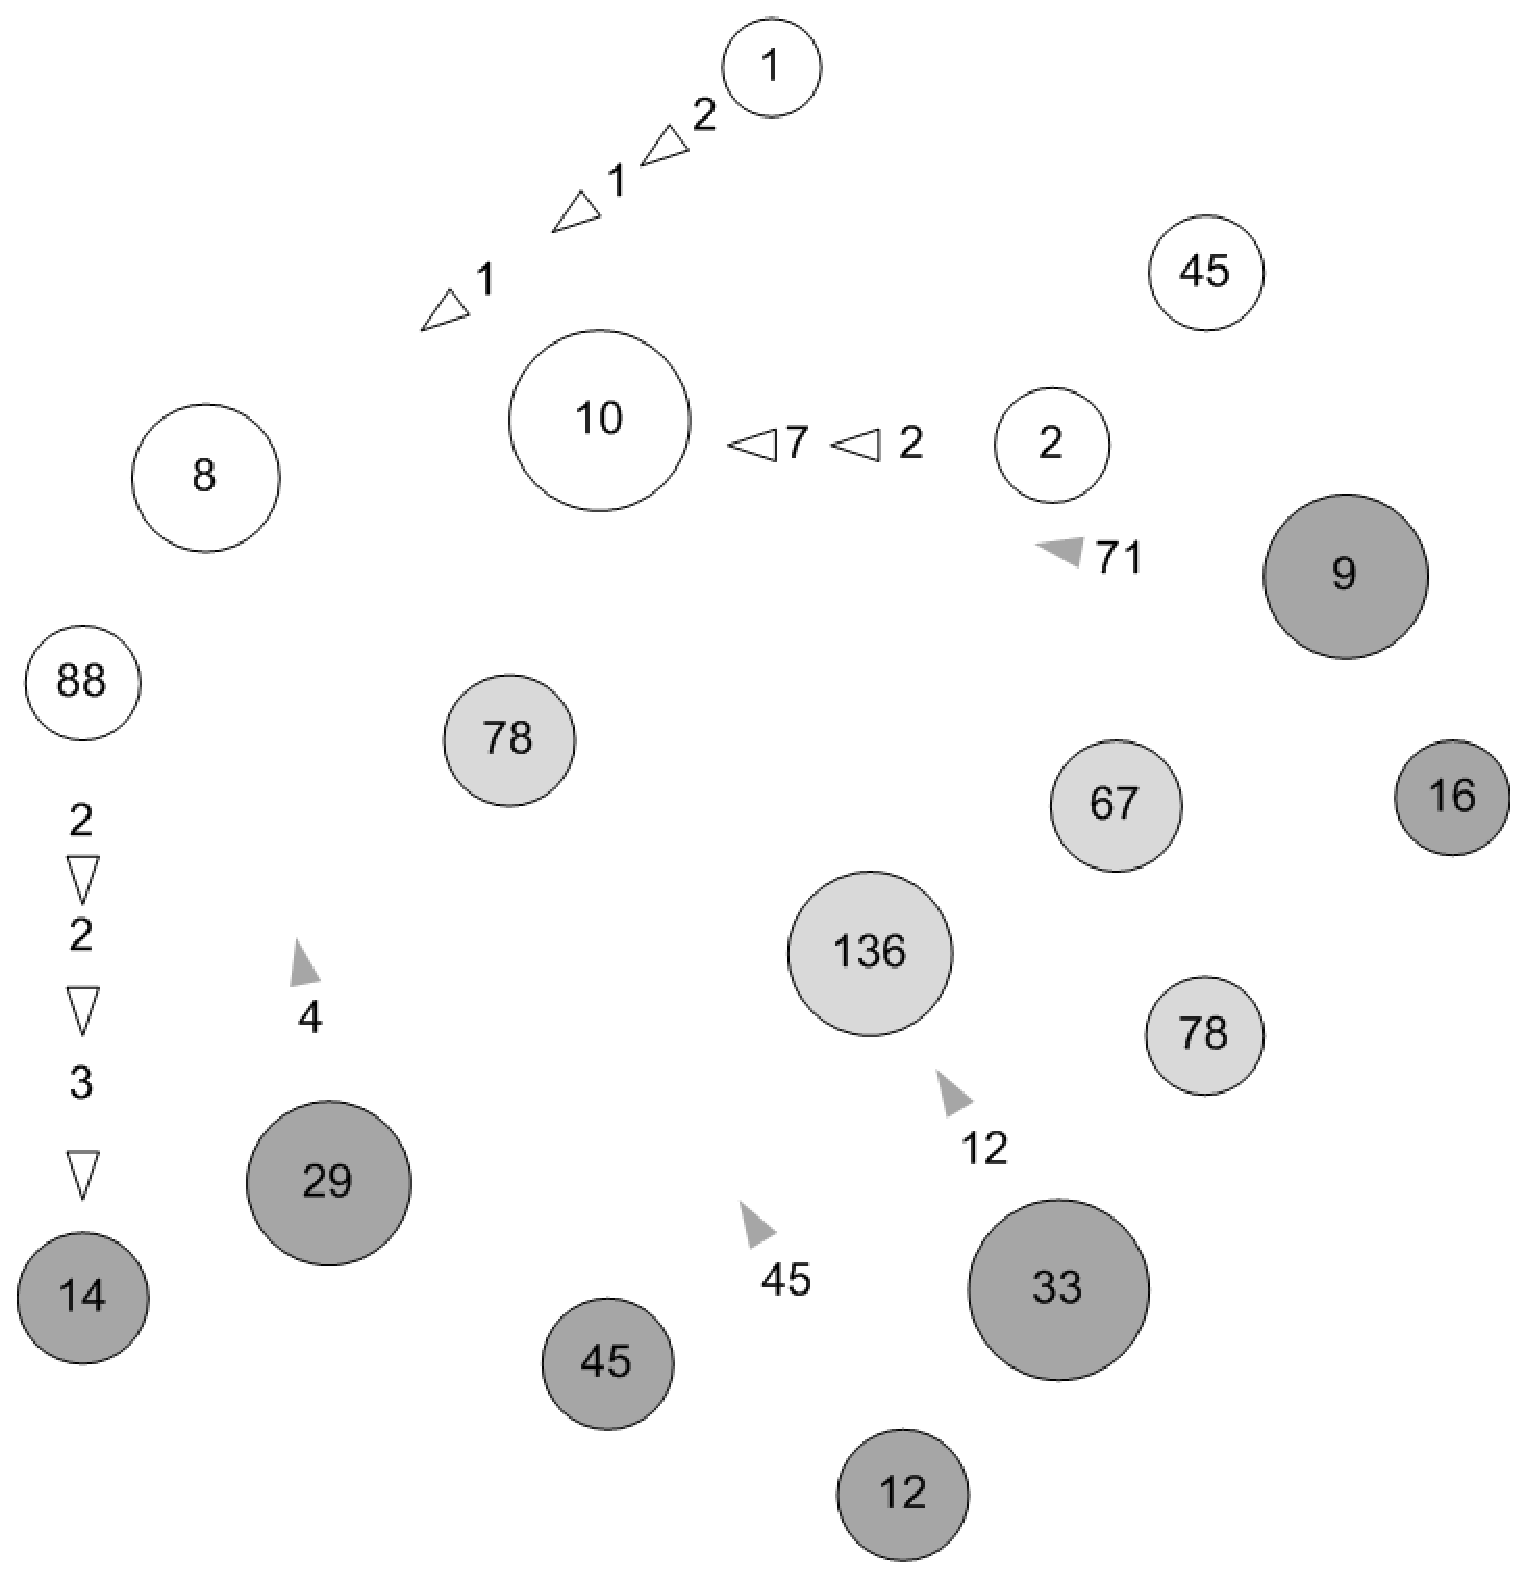
\epsfig{file=./imagenes/naves.eps,width=4cm}
\end{center}
\caption{Simulated screen shot of an early stage of a run in Planet Wars. White planets belong to the player (blue colour in the game), dark grey belong to the opponent (red in the game), and light grey planets belong to no player. The triangles are fleets, and the numbers (in planets and triangles) represent the ships. The planet size means growth rate of the amount of ships in it (the bigger, the higher).}
\label{figura:PlanetWars1}
\end{figure}

A Planet Wars match takes place on a map (see Figure \ref{figura:PlanetWars1}) that contains several planets (neutral, enemies or owned), each one of them with a number assigned to it that represents the quantity of ships that the planet is currently hosting. 

The aim of the game is to defeat all the ships in the opponent's planets. Although Planet Wars is a RTS game, this implementation has transformed it into a turn-based game, in which each player has a maximum number of turns to accomplish the objective. At the end of the match the winner is the player live, or owning more ships if more than one survives. 

There are two strong constraints which determine the possible methods to apply to design
a bot: a simulated turn takes \textit{just one second}, and the bot is \textit{not allowed to store any kind of information} about its former actions, about the opponent's actions or about the state of the game (i.e., the game's map).

Therefore, the goal in this paper is to study the improve of a bot, ---------- according to the state of the map in each simulated turn (input) returns a set of actions to perform in order to fight the enemy, conquer its resources, and, ultimately, win the game. In the original game, only two bots are faced but in this paper it's studied what happen when we simulated 4 on 4 battles, it's mean, when 4 bots are fighting in the same map.


%%%%%%%%%%%%%%%%%%%%%%%%%%%%%%%%  CO-EVOLUTION  %%%%%%%%%%%%%%%%%%%%%%%%%%%%%%%%
%
\section{Cooperative and Competitive Evolution: Co-evolution}
\label{sec:co-genebot}

%Añadir referencias de Maribel:

There are two types of co-evolutions, attend of the interaction between the individuals of the population: cooperative and competitive. In this paper, it's described an coevolutionary algorithm that has the two sides.

For one hand, are will simulated 4 on 4 battles were severals bots will fight for the same goal: win the battle. That means that the bots will compete against each other. Also, the individuals are competing in the GA for perpetuate their species.

For other hand, the cooperative side come because the 4 on 4 battle is {$all\ versus\ all$}, so a single individual may have help of others for {$kill$} a temporally mutual rival. But beware, it's totally sure that at the end, can be only one. In addition, in the GA the individuals are sharing {$knowledge$}, because they are {$living$} (and fighting) together. If the population is each time better, and the new individuals are {$born$} of these population, the new individuals will be better and better.

One of the major problems founded in the use of EAs for training bots for this behavior was the huge time needed for the evaluation, because we have to simulated fulls battles, in several maps, several times causes. In addition, when dealing with a noise and stochastic problem like this, it's forced to use re-evaluation between generations.

Theoretically, the use of a co-evolution allow to reduce the number of simulations needed, because the population it's evaluated in {$groups$}. That's, if there are a population of 100 individuals, in a classic GA it's needed make 100 evaluations, once for each individual, for each generation, times for the number of maps and the re-evaluation or others factors. In co-evolution case, for example, if it's used 2 bots of the population for the co-evolution it's only need 50 evaluations for the Co-GA. It's likely that simulations with 4 bots will take more time that a simulation with 2 bots, but the question is if the time taken for a {$4-simulations$} is less that the time taken for two {$2-simulation$}. In that case, the co-evolution will decrease the time needed for the training.

The use of 2 individuals or 4 individuals of the population in the experiments depends of the use (or not) of previous knowledge. 

\subsection{Previous Knowledge vs Auto-generated Knowledge}
\label{sec:knowledge}

It has an best training bot, which has proved its worth in 1vs1 battles. The question is if can be used the previous knowledge for improve (faster) better bots in a similar problem. Or maybe, if it's best don't use previous knowledge and allow fight versus individuals of the population; that theoretically (as the bases of the GAs) will be better and better in each generation. To answer this question, were making two types of experiments.

\subsubsection{Co-evolution with previous Knowledge}
\label{sec:knowledge:previous}

In this case, will be simulated battles between two individuals of the population versus two of the best bots (in 1vs1 contest). It's expected that the co-bots can learn the bases of the best bots, and improve for be better in 4 on 4 battles. It's desirable that this type of co-evolution prize bots that at least can win in a battled of the previous best bots.

Talcking about the time needed for the execution, it's not expected an huge reduction of the time needed for the training of the bots, but it's desirable that happen. It's something that will be increased in the next co-evolution method.

\subsubsection{Co-evolution with Auto-generated Knowledge}
In this case, will be simulated battles between four individuals of the population. It's not used previous knowledge of previous works, but the bots were improving for be better versus bots every time betters (because it's expected that the population will better in each generation).

Talcking about the time, this method would reduce the time needed near to 50\% that the previous method, because it reduced the number of evaluations to the half.

\subsection{Fitness}

In previous works, it's evaluated a single bot of the population versus always the same bot (an reference-bot). For fitness function, the bot was evaluated several times (in different maps). The fitness function was defined depending of the result of the battle (if the bot wins all his battles or loses in someone) and the numbers of turns needed for end the game. For two bots A and B the fitness is defined like show in Fig.\ref{fig:fitness_turns_positions} \subref{fig:fitness_turns_positions:2}. 

%This fitness works well for 1vs1 battles, and the first fitness proposed is an natural evolution of this fitness applied to 4 on 4 bots battles.

\subsubsection{Fitness based in Position and turns}

This fitness it's an natural evolution of the previous, applied to 4 bots battles. Again, the evaluations are in several maps. In this case, it's studied the position ($1^{th}$, $2^{th}$,..) of the bot in the 4-battle and the number of turns. For a bot that wins all the battles (it's $1^{th}$ in all) it's call {$ferocity$} to the sum turns, in previous works was found that a bot that wins in less turns it's best that other that takes more turns in win too. In other case, the sum of turns it's call {$sturdy$}, and opposite to the {$ferocity$}, it's desirable a bot that take more turns in be defeated. In fig\ref{fig:fitness_turns_positions}(\subref{fig:fitness_turns_positions:2})there are an formal description of this fitness.

\begin{figure}[h]
\tiny
\begin{subfigure}[!]{0.5\textwidth}
\begin{algorithmic}
        \State{$A,B\in Population $}
        \If {A WINs always}
            \If{B LOSEs some battle}
                \State A is better than B
            \ElsIf{A take less turns than B}
                \State A is better than B
            \Else
                \State B is better than A
            \EndIf
        \Else
             \If{B WINs always}
                \State B is better than A
            \ElsIf{A take less turns than B}
                \State B is better than A
            \Else
                \State A is better than B
            \EndIf
        \EndIf
        \end{algorithmic}
        \label{fig:fitness_turns_positions:2}
\caption{Fitness used in battles of 2 bots}
\end{subfigure}
\begin{subfigure}[!]{0.5\textwidth}
    \begin{algorithmic}
        \State{$A,B\in Population $}
        \If {A average position $<$ B average position}
            \State A is better than B
        \ElsIf{A average position $>$ B average position}
            \State B is better than A
        \Else
            \If{A,B is always $1^{th}$}
                \If{A take less turns than B}
                    \State A is better than B
                \Else
                    \State B is better than A
                \EndIf
            \Else
                \If{A take less turns than B}
                    \State B is better than A
                \Else
                    \State A is better than B
                \EndIf
            \EndIf
        \EndIf
    \end{algorithmic}
    \label{fig:fitness_turns_positions:co}
\caption{Fitness used in battles of 4 bots}
\end{subfigure}
\label{fig:fitness_turns_positions}
\caption{Fitness based in turns and positions}
\end{figure}

In this fitness, we are only interesting in the final result: position and turn. We aren't student how the bot reach it. However, two variables are involved in the calculation of the fitness. That difficult the operation with severals evaluations, because the fitness can't be easily sum o averaged. In the next fitness, it's used another metric to define the goodness of the bots. The percentage of the ships that in each turn belong to each player. 

For study the ships, it's taken from the simulation how many ships belong to each player in each turn, normalized at total ships in game for that turn (including neutrals ships in neutral planets). For each player, we have a {$cloud$} different like in Fig.\ref{figura:nubecita}. Below, see two alternatives to deal with this cloud of points for the fitness function: using slopes and areas.

\begin{figure}[h]
\begin{center}
  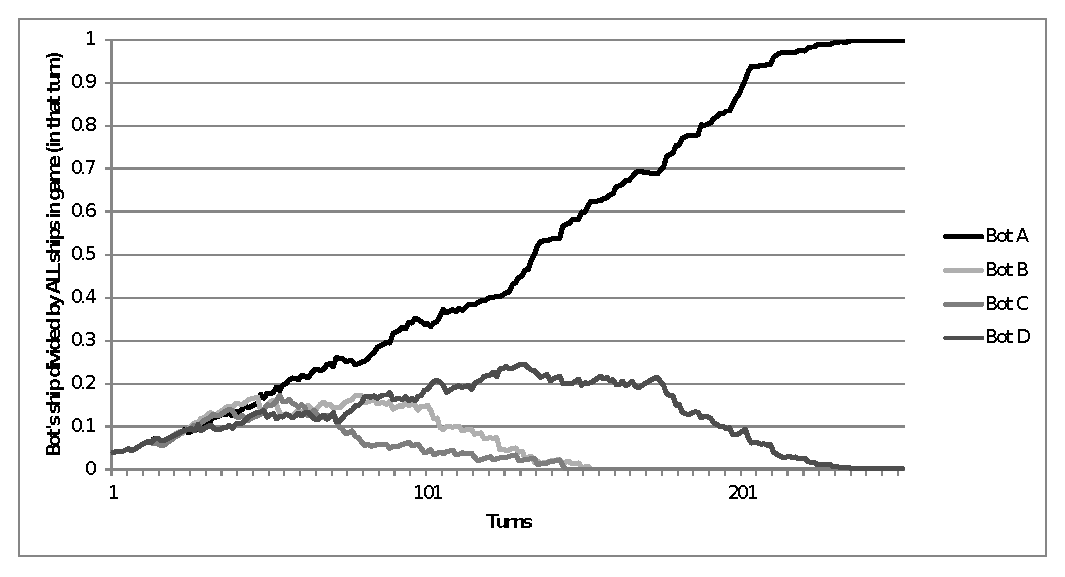
\epsfig{file=imagenes/nubecita.eps,width=4cm}
\end{center}
\caption{Representation of the number if ships of each bot in each turn} 
\label{figura:nubecita}
\end{figure}

\subsubsection{Fitness based in Slope}

For this fitness, it's used the least squares regression analysis for resume the cloud of points to a simple line. A line is represented as {$y = \alpha \times x + \beta $}, where {$\alpha$} and {$\beta$} are calculated as show the Fig. \ref{equation:LeatsSqueares} according to least squares regression. For each bot in the simulation it's calculated $\alpha$, that it's also call $slope$. This $slope$ it's the fitness defined for each bot for that simulation.

\begin{figure}[h]
\begin{subfigure}[H]{0.4\textwidth}
    \begin{equation}
        \alpha = \frac{\sum_{i=1}^{n}(X_{i} - \bar{X_{i}})(Y_{i} - \bar{Y_{i}})}{\sum_{i=1}^{n}(X_{i} - \bar{X_{i}})^{2}}
    \end{equation}
    \begin{equation}
        \beta = \bar{Y}-\alpha\bar{X}
    \end{equation}
    \caption{Leats squares regression}
    \label{equation:LeatsSqueares}
\end{subfigure}
\begin{subfigure}[H]{0.8\textwidth}
\begin{center}
  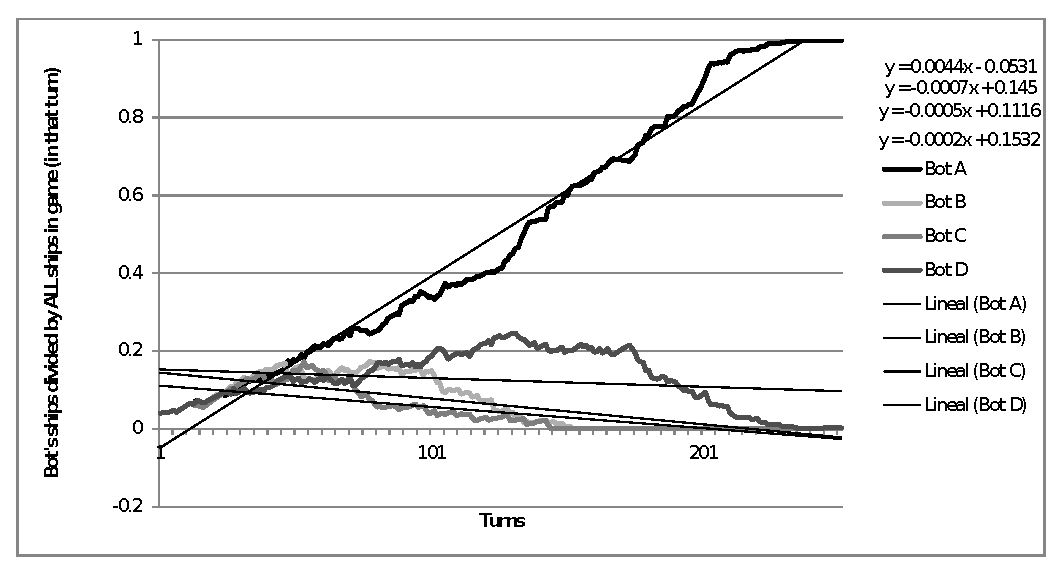
\epsfig{file=imagenes/nubecita_pendiente.eps,width=1\textwidth}
\end{center}
\caption{Representation of the number if ships of each bot in each turn} 
\label{figura:nubecita}
\end{subfigure}
\end{figure}

Can be establish an theoretical maximal an minimal values for this fitness. An hypothetical bot that wins in the first turn, will have an slope of {$1$}, so this is the maximal value of our fitness. For other hand, an bot that loses in the first turn, will have an slope of {$-1$}. In addition, looking at the slope, can be known if the bot {$WINs$} ({$slope>0$}) or {$LOSEs$} {$slope<0$}. Finally, can be determined that when the slope was greater (and therefore closer to the maximum) should be better the bot.

Several evaluations in different maps was using, so it's need operate with fitness. In that case, only sum the slope of all the evaluations of the bot.

\subsection{Fitness bases in Area}
\label{sec:fitness}

In these fitness, it's used the integral of the curve for calculate the area between it and the x-axis. This {$area$} is normalized to the number of turns, representing the average percentage of ships along the battle for each player. In the Fig\subref{equation:LeatsSqueares}

\begin{figure}[h]
\begin{subfigure}[H]{0.4\textwidth}
    \begin{equation}
        area=\frac{\int_{0}^{t}\%ships(x)dx}{t}
    \end{equation}
    \caption{Calculus of the area}
    \label{equation:LeatsSqueares}
\end{subfigure}
\begin{subfigure}[H]{0.8\textwidth}
\begin{center}
  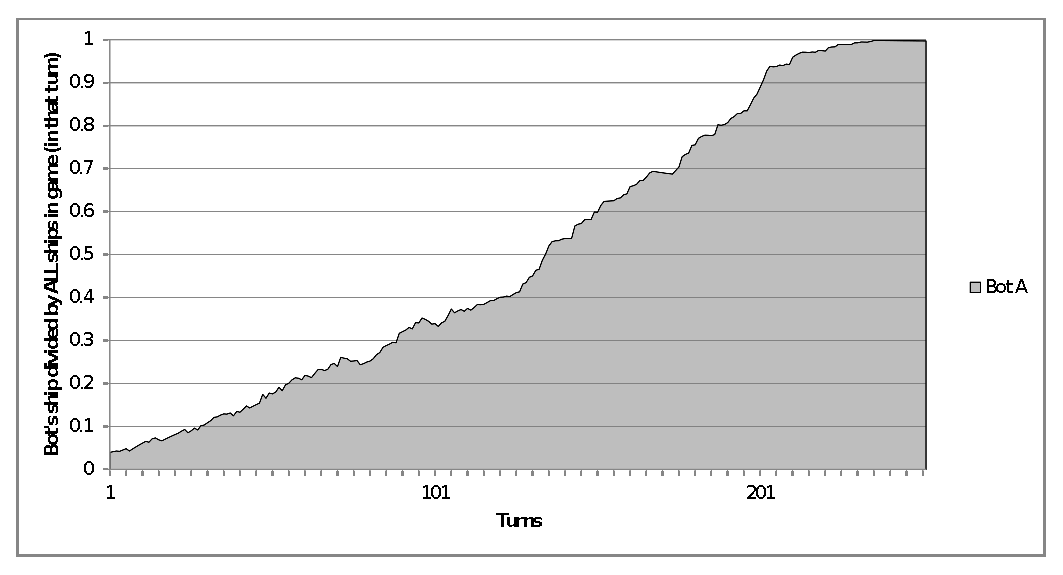
\epsfig{file=imagenes/nubecita_integral.eps,width=1\textwidth}
\end{center}
\caption{Example of area under the curve} 
\label{figura:nubecita}
\end{subfigure}
\end{figure}

As before, can be established an theoretical maximal an minimal values for this fitness. An hypothetical bot that wins in the first turn, will have an area closer to {$1$}, so this is the maximal value of the fitness. Furthermore, an bot that loses in the first turn, will have an area near to {$0$}. In this case, can't be know by the fitness if the bot wins or loses the battle. In this scope, we are losing information.

%%%%%%%%%%%%%%%%%%%%%%%%%%%%%%%   EXPERIMENTS  %%%%%%%%%%%%%%%%%%%%%%%%%%%%%%%%
%
\section{Experiments and Results}
\label{sec:experiments}


%%%%%%%%%%%%%%%%%%%%%%%%%%%%%%  CONCLUSIONS  %%%%%%%%%%%%%%%%%%%%%%%%%%%%%%%
%
\section{Conclusions and Future Work}
\label{sec:conclusions}



%%%%%%%%%%%%%%%%%%%%%%%%%%%%%%   ACKNOWLEDGEMENTS %%%%%%%%%%%%%%%%%%%%%%%%%%%%%%

\section*{Acknowledgements}

This paper has been funded in part by projects P08-TIC-03903 (Andalusian Regional Government), TIN2011-28627-C04-02 (Spanish Ministry of Science and Innovation), and project 83 (CANUBE) awarded by the CEI-BioTIC UGR.

\bibliographystyle{splncs}
\bibliography{genebot}


\end{document}
